\chapter{Discussion}
Please tell more about conclusion and how to the next work of this study.

\section{Ahmad Syafrizal Huda/1164062}
\subsection{Teori}
\begin{enumerate}
\item Jelaskan kenapa file teks harus di lakukan tokenizer.
\subitem Tokenizer adalah untuk membuat vektor dari teks. Dan mengapa harus dilakukan tokenizer pada file teks? itu karena dengan memfungsikan tokenizer, teks dapat divektorkan. Sehingga teks yang telah telah divektorkan tersebut dapat terbaca pada Machine Learning. Proses tokenizer itu hanya memenggal kata-kata yang ada didalam suatu frasa atau kalimat yang terdapat didalam suatu text dataset. Ilustrasi gambar dapat dilihat pada gambar \ref{c7_1}.
\begin{figure}[!htbp]
	\centerline{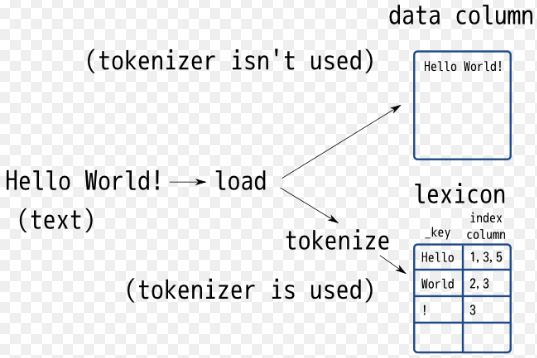
\includegraphics[width=1\textwidth]{figures/huda/chapter7/1.JPG}}
	\caption{Tokenizer}
	\label{c7_1}
\end{figure}
\item Jelaskan konsep dasar K Fold Cross Validation pada dataset komentar Youtube pada kode listing \ref{lst:7.0}.
\begin{lstlisting}[caption=K Fold Cross Validation,label={lst:7.0}]
kfold = StratifiedKFold(n_splits=5)
splits = kfold.split(d, d['CLASS'])
\end{lstlisting}
\subitem StartifiedKFold berisikan presentasi sampel untuk setiap kelas. Dimana dalam ilustrasi ini sampel dibagi menjadi 5 dalam setiap class nya. Kemudian sampel tadi akan dimasukan kedalam class dari dataset youtube tadi. Contoh dapat dilihat pada gambar \ref{c7_2}.
\begin{figure}[!htbp]
	\centerline{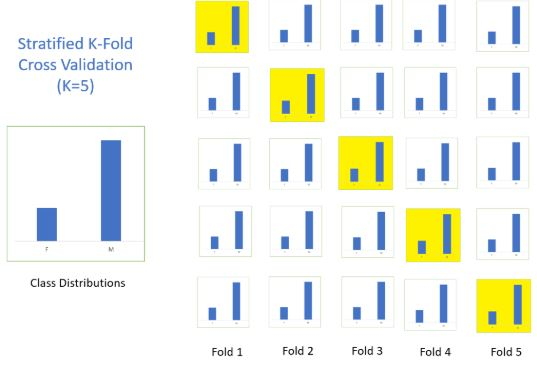
\includegraphics[width=1\textwidth]{figures/huda/chapter7/2.JPG}}
	\caption{StartifiedKFold}
	\label{c7_2}
\end{figure}
\item Jelaskan apa maksudnya kode program for train, test in splits.
\subitem Maksudnya yaitu untuk menguji apakah setiap data pada dataset sudah di split dan tidak terjadi penumpukan. Yang dimana maksudnya di setiap class tidak akan muncul id yang sama. Ilustrasinya misalkan kita memiliki 4 baju dengan model yang berbeda. Kemudian kita bagikan kedua anak, tentunya setiap anak yang menerima baju tidak memiliki baju yang sama modelnya.
\item Jelaskan apa maksudnya kode program \emph{train\_content = d['CONTENT'].iloc[train\_idx]} dan \emph{test\_content = d['CONTENT'].iloc[test\_idx]}.
\subitem Maksudnya yaitu mengambil data pada kolom atau index CONTENT yang merupakan bagian dari train\_idx dan test\_idx. Ilustrasinya, ketika data telah diubah menjadi train dan test maka kita dapat memilihnya untuk ditampilkan pada kolom yang diinginkan.
\item Jelaskan apa maksud dari fungsi \emph{tokenizer = Tokenizer(num\_words=2000)} dan \emph{tokenizer.fit\_on\_texts(train\_content)}.
\subitem Dimana variabel tokenizer akan melakukan vektorisasi kata menggunakan fungsi Tokenizer yang dimana jumlah kata yang ingin diubah kedalam bentuk token adalah 2000 kata. Dan untuk \emph{tokenizer.fit\_on\_texts(train\_content)} maksudnya kita akan melakukan fit tokenizer hanya untuk dat trainnya saja tidak dengan data test nya untuk kolom CONTENT. Ilustrasinya, Jadi, jika Anda memberikannya sesuatu seperti, "Kucing itu duduk di atas tikar." Ini akan membuat kamus s.t. word\_index ["the"] = 0; word\_index ["cat"] = 1 itu adalah kata -> kamus indeks sehingga setiap kata mendapat nilai integer yang unik.
\item Jelaskan apa maksud dari fungsi \emph{d\_train\_inputs = tokenizer.texts\_to\_matrix(train\_content, mode='tfidf')} dan \emph{d\_test\_inputs = tokenizer.texts\_to\_matrix(test\_content, mode='tfidf')}.
\subitem Maksudnya yaitu untuk variabel d\_train\_inputs akan melakukan tokenizer dari bentuk teks ke matrix dari data train\_content dengan mode matriksnya yaitu tfidf begitu juga dengan variabel d\_test\_inputs untuk data test. Contoh dapat dilihat pada gambar \ref{c7_3}.
\begin{figure}[!htbp]
	\centerline{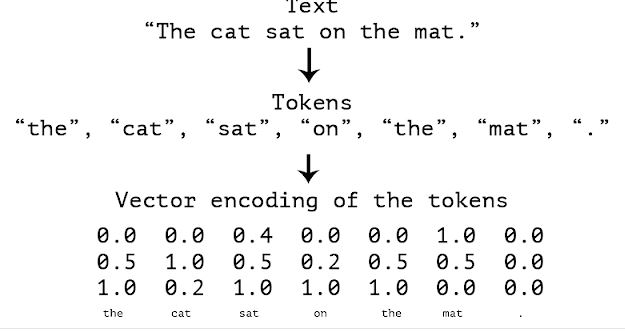
\includegraphics[width=1\textwidth]{figures/huda/chapter7/3.JPG}}
	\caption{Fungsi Tokenizer}
	\label{c7_3}
\end{figure}
\item Jelaskan apa maksud dari fungsi \emph{d\_train\_inputs = d\_train\_inputs/np.amax(np.absolute(d\_train\_inputs))} dan \emph{d\_test\_inputs = d\_test\_inputs/np.amax(np.absolute(d\_test\_inputs))}.
\subitem Fungsi tersebut akan membagi matrix tfidf tadi dengan amax yaitu mengembalikan maksimum array atau maksimum sepanjang sumbu. Yang hasilnya akan dimasukan kedalam variabel d\_train\_inputs untuk data train dan d\_test\_inputs untuk data test dengan nominal absolut atau tanpa ada bilangan negatif dan koma. Contoh dapat dilihat pada gambar\ref{c7_4}.
\begin{figure}[!htbp]
	\centerline{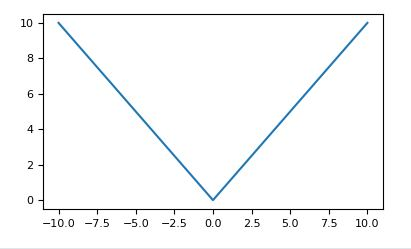
\includegraphics[width=1\textwidth]{figures/huda/chapter7/4.JPG}}
	\caption{Matrix TFID}
	\label{c7_4}
\end{figure}
\item Jelaskan apa maksud fungsi dari d train outputs = np utils.to categorical(d['CLASS'].iloc[train dan d test outputs = np utils.to categorical(d['CLASS'].iloc[test idx]) dalam kode program.
\subitem maksud dari fungsi tersebut yaitu untuk merubah nilai vektor yang ada pada atribut class menjadi bentuk matrix dengan pengurutan berdasarkan data index training dan testing. Contoh dapat dilihat pada gambar \ref{c7_5}
\begin{figure}[!htbp]
	\centerline{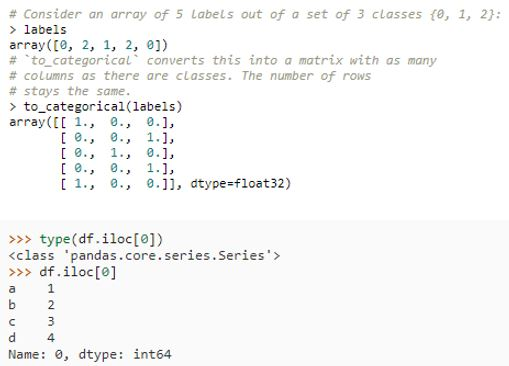
\includegraphics[width=1\textwidth]{figures/huda/chapter7/5.JPG}}
	\caption{Matrix Training dan Testing}
	\label{c7_5}
\end{figure}
\item Jelaskan apa maksud dari fungsi di listing \ref{lst:7.1}. Gambarkan ilustrasi Neural Network nya dari model kode tersebut.
\begin{lstlisting}[caption=Neural Network,label={lst:7.1}]
model=Sequential()
model.add(Dense(512,input_shape=(2000,)))
model.add(Activation('relu'))
model.add(Dropout(0.5))
model.add(Dense(2))
model.add(Act ivation('softmax'))
\end{lstlisting}
\item Jelaskan apa maksud dari fungsi di listing \ref{lst:7.2} dengan parameter tersebut.
\begin{lstlisting}[caption=Model Compile Metric,label={lst:7.2}]
model . compile(loss='categorical_crossentropy',optimizer='adamax',
metrics=[ 'accuracy '])
\end{lstlisting}
\item Jelaskan apa itu Deep Learning.
\subitem Deep Learning merupakan cabang dari Machine Learning atau bagian keluarga yang lebih luas dari method machine learning berdasarkan pada representasi data pembelajaran dan memiliki konsep serupa, tapi dilakukan dengan metode yang lebih cerdas. Deep Learning menggunakan Deep Neural Network dalam menyelesaikan suatu masalah yang terjadi pada Machine Learning.
\item Jelaskan apa itu Deep Neural dan bedanya dengan Deep Learning.
\begin{itemize}
\item Deep Neural Network atau DNN merupakan algoritma yang berbasis neural network yang digunakan untuk mengambil keputusan.
\item Yang membedakan Deep Learning dengan  Deep Neural Network (DNN) adalah DNN merupakan algoritma yang digunakan pada Deep Learning, sedangkan Deep Learning merupakan model yang menggunakan algoritma DNN.
\end{itemize}
\item Jelaskan dengan ilustrasi gambar buatan sendiri(langkah per langkah) bagaimana perhitungan algoritma konvolusi dengan ukuran stride (NPM mod3+1) x (NPM mod3+1) yang terdapat max pooling.
\subitem Konvolusi pada gambar dilakukan dalam image processing untuk menerapkan operator yang memiliki nilai output dari piksel gambar yang berasal dari kombinasi linear nilai input piksel, semakin nilai piksel tersebut maka kualitas gambar bisa semakin bagus. Contoh ilustrasi gambar dapat dilihat pada gambar \ref{c7_6} dan \ref{c7_7}.
\begin{figure}[!htbp]
	\centerline{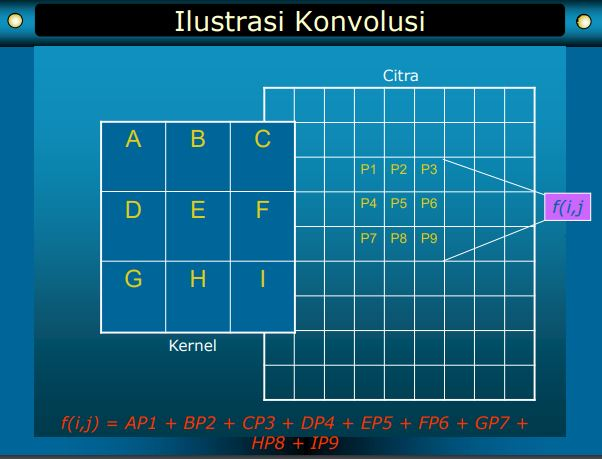
\includegraphics[width=1\textwidth]{figures/huda/chapter7/6.JPG}}
	\caption{Konvolusi}
	\label{c7_6}
\end{figure}
\begin{figure}[!htbp]
	\centerline{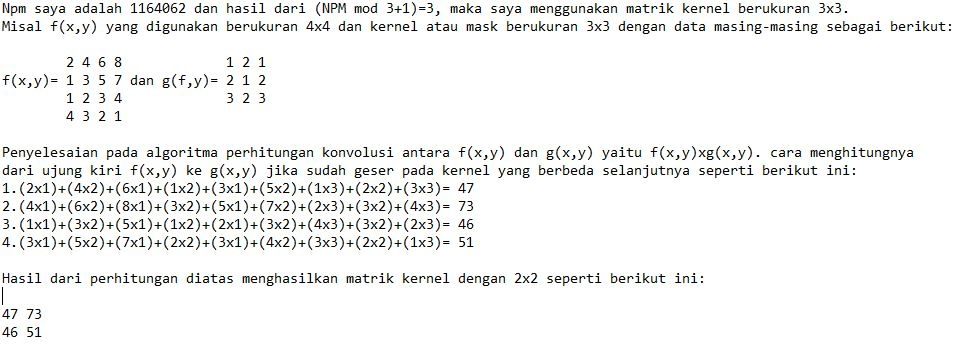
\includegraphics[width=1\textwidth]{figures/huda/chapter7/7.JPG}}
	\caption{Algoritma Perhitungan Konvolusi}
	\label{c7_7}
\end{figure}
\end{enumerate}

\subsection{Praktek Program}
\begin{enumerate}
\item Jelaskan kode program pada blok \# In[1]
\par Berikut adalah kode program yang digunakan :
\lstinputlisting[firstline=2, lastline=4, caption=Kode Program 1, label={1}]{src/MathSymbols.py}
\par Dari kode listing pada kode program 1, dapat dijelaskan seperti berikut :
\begin{itemize}
\item Baris 1	: Melakukan pengimportan file csv
\item Baris 2	: Melakukan pemanggilan atau memasukkan module image sebagai pil\_image dari library PIL
\item Baris 3	: Melakukan pengimportan fungsi keras.processing.image 
\end{itemize}
\par Sehingga dari kode program tersebut bila dijalankan, maka menghasilkan seperti pada gambar \ref{c7_8}.
\begin{figure}[!htbp]
	\centerline{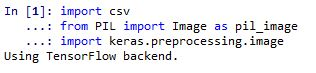
\includegraphics[width=1\textwidth]{figures/huda/chapter7/8.JPG}}
	\caption{In[1]}
	\label{c7_8}
\end{figure}
\item Jelaskan kode program pada blok \# In[2]
\par Berikut adalah kode program yang digunakan :
\lstinputlisting[firstline=8, lastline=21, caption=Kode Program 2, label={2}]{src/MathSymbols.py}
\par Dari kode listing pada kode program 2, dapat dijelaskan seperti berikut :
\begin{itemize}
\item Baris 1	: Membuat variabel imgs tanpa ada parameter di dalamnya
\item Baris 2	: Membuat variabel classes tanpa ada parameter didalamnya
\item Baris 3	: Membuka file csv dari HASYv2/hasy-data-labels.csv sebagai csvfile
\item Baris 4	: Membuat variabel csvreader yang difungsikan untuk membaca dari file csv yang dimasukkan
\item Baris 5	: Membuat variabel i dengan parameter 0 atau nilai 0
\item Baris 6	: Digunakan untuk melakukan eksekusi baris dari pembacaan csv 
\item Baris 7	: Mengaplikasikan atau menggunakan perintah "if" dengan variabel i lebih besar dari 0, yang selanjutnya akan dilanjutkan ke perintah berikutnya
\item Baris 8	: Membuat variabel img yang berfungsi untuk mengubah image atau gambar menjadi bentuk array (bilangan) dari file HASYv2 yang dibuka dengan row berparameter 0.
\item Baris 9	: Membuat variabel img dengan nilai bukan sama dengan 255.0
\item Baris 10 : Mendefinisikan fungsi imgs.append yang digunakan untuk melakukan proses penggabungan data dengan file lain atau dataset lain yang telah ditentukan dengan 3 parameter yaitu row[0], row[2] dan variabel img.
\item Baris 11 : Mendefinisikan fungsi append dari variabel classes dengan menggunakan parameter row[2].
\item Baris 12 : Mengartikan i=i+1 yang dimana nilai sari variabel i akan ditambah 1 sehingga akan bernilai 1.
\end{itemize}
\par Sehingga dari kode program tersebut bila dijalankan, maka menghasilkan seperti pada gambar \ref{c7_9}.
\begin{figure}[!htbp]
	\centerline{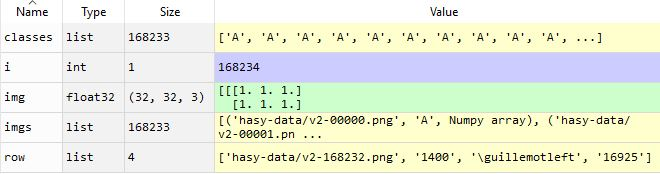
\includegraphics[width=1\textwidth]{figures/huda/chapter7/9.JPG}}
	\caption{In[2]}
	\label{c7_9}
\end{figure}
\item Jelaskan kode program pada blok \# In[3]
\par Berikut adalah kode program yang digunakan :
\lstinputlisting[firstline=25, lastline=29, caption=Kode Program 3, label={3}]{src/MathSymbols.py}
\par Dari kode listing pada kode program 3, dapat dijelaskan seperti berikut :
\begin{itemize}
\item Baris 1	: Memanggil dan menggunakan module random
\item Baris 2	: Melakukan pengocokan menggunakan module random pada parameter variabel imgs
\item Baris 3	: Membagi index data kedalam bentuk integer dengan mengalikan 0,8 dan len yang berfungsi mengembalikan jumlah item dalam datanya dari variabel imgs
\item Baris 4	: Membuat variabel train yang digunakan untuk mengeksekusi imgs serta pemecahan index awal pada data untuk digunakan sebagai data training
\item Baris 5	: Membuat variabel test yang digunakan untuk mengeksekusi imgs serta pemecahan index akhir pada data untuk digunakan sebagai data testing
\end{itemize}
\par Sehingga dari kode program tersebut bila dijalankan, maka menghasilkan seperti pada gambar \ref{c7_10}.
\begin{figure}[!htbp]
	\centerline{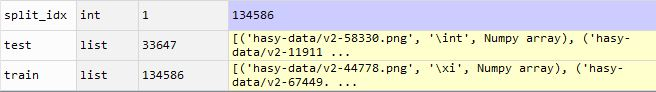
\includegraphics[width=1\textwidth]{figures/huda/chapter7/10.JPG}}
	\caption{In[3]}
	\label{c7_10}
\end{figure}
\item Jelaskan kode program pada blok \# In[4]
\par Berikut adalah kode program yang digunakan :
\lstinputlisting[firstline=33, lastline=39, caption=Kode Program 4, label={4}]{src/MathSymbols.py}
\par Dari kode listing pada kode program 4, dapat dijelaskan seperti berikut :
\begin{itemize}
\item Baris 1	: Melakukan import library numpy sebagai np
\item Baris 2	: Membuat variabel train\_input untuk mengubah inputan menjadi array menggunakan fungsi np.asarray dan  fungsi list untuk mengkoleksi data yang dipilih serta data dapat diubah. Dan didalamnya melakukan penerapan fungsi map yang berfungsi untuk mengembalikan iterator dari data yang digunakan dan fungsi lamda pada row berparameter [2] difungsikan untuk membuat objek menjadi lebih kecil sehingga mudah dieksekusi dari variabel train.
\item Baris 3	: Membuat variabel test\_input untuk mengubah inputan menjadi array menggunakan fungsi np.asarray dan  fungsi list untuk mengkoleksi data yang dipilih serta data dapat diubah. Dan didalamnya melakukan penerapan fungsi map yang berfungsi untuk mengembalikan iterator dari data yang digunakan dan fungsi lamda pada row berparameter [2] difungsikan untuk membuat objek menjadi lebih kecil sehingga mudah dieksekusi dari variabel test.
\item Baris 4	: Membuat variabel train\_input untuk mengubah inputan menjadi array menggunakan fungsi np.asarray dan  fungsi list untuk mengkoleksi data yang dipilih serta data dapat diubah. Dan didalamnya melakukan penerapan fungsi map yang berfungsi untuk mengembalikan iterator dari data yang digunakan dan fungsi lamda pada row berparameter [1] difungsikan untuk membuat objek menjadi lebih kecil sehingga mudah dieksekusi dari variabel train.
\item Baris 5	: Membuat variabel test\_input untuk mengubah inputan menjadi array menggunakan fungsi np.asarray dan  fungsi list untuk mengkoleksi data yang dipilih serta data dapat diubah. Dan didalamnya melakukan penerapan fungsi map yang berfungsi untuk mengembalikan iterator dari data yang digunakan dan fungsi lamda pada row berparameter [1] difungsikan untuk membuat objek menjadi lebih kecil sehingga mudah dieksekusi dari variabel test.
\end{itemize}
\par Sehingga dari kode program tersebut bila dijalankan, maka menghasilkan seperti pada gambar \ref{c7_11}.
\begin{figure}[!htbp]
	\centerline{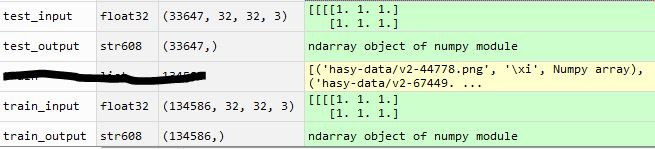
\includegraphics[width=1\textwidth]{figures/huda/chapter7/11.JPG}}
	\caption{In[4]}
	\label{c7_11}
\end{figure}
\item Jelaskan kode program pada blok \# In[5]
\par Berikut adalah kode program yang digunakan :
\lstinputlisting[firstline=42, lastline=43, caption=Kode Program 5, label={5}]{src/MathSymbols.py}
\par Dari kode listing pada kode program 5, dapat dijelaskan seperti berikut :
\begin{itemize}
\item Baris 1	: Menggunakan fungsi LabelEncoder dari sklearn.processing yang berfungsi untuk menormalkan label dimana label encoder hanya didefinisikan dengan nilai antara 0 dan -1.
\item Baris 2	: Menggunakan fungsi OneHotEncoder dari sklearn.processing yang berfungsi untuk mendefinisikan fitur input yang dimana mengambil nilai dalam kisaran [0, nilai maksimal].
\end{itemize}
\par Sehingga dari kode program tersebut bila dijalankan, maka menghasilkan seperti pada gambar \ref{c7_12}.
\begin{figure}[!htbp]
	\centerline{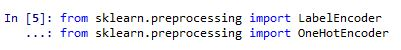
\includegraphics[width=1\textwidth]{figures/huda/chapter7/12.JPG}}
	\caption{In[5]}
	\label{c7_12}
\end{figure}
\item Jelaskan kode program pada blok \# In[6]
\par Berikut adalah kode program yang digunakan :
\lstinputlisting[firstline=48, lastline=49, caption=Kode Program 6, label={6}]{src/MathSymbols.py}
\par Dari kode listing pada kode program 6, dapat dijelaskan seperti berikut :
\begin{itemize}
\item Baris 1	: Membuat variabel label\_encoder dengan penerapan modul / fungsi LabelEncoder tanpa parameter
\item Baris 2	: Membuat variabel integer\_encoded dengan penerapan fungsi label\_encoder.fit\_transform yang berfungsi untuk melakukan ekstrasi fitur object dari variabel classes yang akan mengembalikan beberapa data yang diubah kembali.
\end{itemize}
\par Sehingga dari kode program tersebut bila dijalankan, maka menghasilkan seperti pada gambar \ref{c7_13}.
\begin{figure}[!htbp]
	\centerline{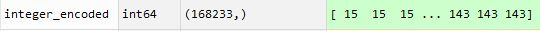
\includegraphics[width=1\textwidth]{figures/huda/chapter7/13.JPG}}
	\caption{In[6]}
	\label{c7_13}
\end{figure}
\item Jelaskan kode program pada blok \# In[7]
\par Berikut adalah kode program yang digunakan :
\lstinputlisting[firstline=52, lastline=54, caption=Kode Program 7, label={7}]{src/MathSymbols.py}
\par Dari kode listing pada kode program 7, dapat dijelaskan seperti berikut :
\begin{itemize}
\item Variabel onehot\_encoder akan memanggil fungsi OneHotEncoder dimana tidak berisikan matriks sparse.
\item Pada variabel integer\_encoded akan diubah bentuknya dimana setiap nilai integer akan direpresentasikan sebagai vektor binari dengan nilai 0 kecuali index dari integer tersebut ditandai dengan 1.
\item Melakukan fit untuk one hot encoder kedalam integer\_encoder.
\end{itemize}
\par Sehingga dari kode program tersebut bila dijalankan, maka menghasilkan seperti pada gambar \ref{c7_14}.
\begin{figure}[!htbp]
	\centerline{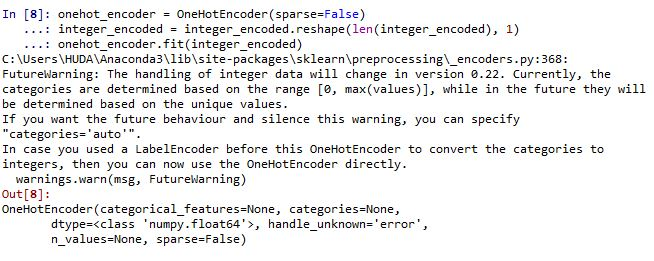
\includegraphics[width=1\textwidth]{figures/huda/chapter7/14.JPG}}
	\caption{In[7]}
	\label{c7_14}
\end{figure}
\item Jelaskan kode program pada blok \# In[8]
\par Berikut adalah kode program yang digunakan :
\lstinputlisting[firstline=57, lastline=63, caption=Kode Program 8, label={8}]{src/MathSymbols.py}
\par Dari kode listing pada kode program 8, dapat dijelaskan seperti berikut :
\begin{itemize}
\item Variabel train\_output\_int  akan mengubah data dari train\_output menjadi LabeEncoder
\item Dimana pada train\_output setelah diubah labelnya menjadi integer dilakukan one hot encoding diambil dari train\_output\_int dan menggunakan .reshape untuk memberikan bentuk baru ke array tanpa mengubah datanya dengan keterangan jika index dari integer tersebut ditandai dengan 1 dan sisanya yang bukan nol.
\item Variabel test\_output\_int  akan mengubah data dari test\_output menjadi LabeEncoder
\item Dimana pada train\_output setelah diubah labelnya menjadi integer dilakukan one hot encoding diambil dari test\_output\_int dan menggunakan .reshape untuk memberikan bentuk baru ke array tanpa mengubah datanya dengan keterangan jika index dari integer tersebut ditandai dengan 1 dan sisanya yang bukan nol.
\item Variabel num\_classes akan menampilakn jumlah data dari classes yang telah dilakukan label encoder
\item Menampilkan tulisan "Number of classes : \%d dmana mengembalikan nilai integer dari num\_classes.
\end{itemize}
\par Sehingga dari kode program tersebut bila dijalankan, maka menghasilkan seperti pada gambar \ref{c7_15}.
\begin{figure}[!htbp]
	\centerline{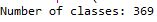
\includegraphics[width=1\textwidth]{figures/huda/chapter7/15.JPG}}
	\caption{In[8]}
	\label{c7_15}
\end{figure}
\item Jelaskan kode program pada blok \# In[9]
\par Berikut adalah kode program yang digunakan :
\lstinputlisting[firstline=67, lastline=69, caption=Kode Program 9, label={9}]{src/MathSymbols.py}
\par Dari kode listing pada kode program 9, dapat dijelaskan seperti berikut :
\begin{itemize}
\item Impor Sequential dari model pada librari Keras.
\item Impor Dense, Dropout, Flatten dari modul Layers pada librari Keras.
\item Impor Conv2D, MaxPooling2D dari modul Layers pada librari Keras.
\end{itemize}
\par Sehingga dari kode program tersebut bila dijalankan, maka menghasilkan seperti pada gambar \ref{c7_16}.
\begin{figure}[!htbp]
	\centerline{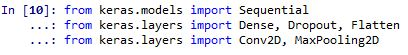
\includegraphics[width=1\textwidth]{figures/huda/chapter7/16.JPG}}
	\caption{In[9]}
	\label{c7_16}
\end{figure}
\item Jelaskan kode program pada blok \# In[10]
\par Berikut adalah kode program yang digunakan :
\lstinputlisting[firstline=71, lastline=85, caption=Kode Program 10, label={10}]{src/MathSymbols.py}
\par Dari kode listing pada kode program 10, dapat dijelaskan seperti berikut :
\begin{itemize}
\item Melakukan pemodelan Sequential.
\item Menambahkan Konvolusi 2D dengan 32 filter konvolusi masing-masing berukuran 3x3 dengan algoritam activation relu dengan data dari train\_input mulai dari baris nol.
\item Menambahkan Max Pooling dengan matriks 2x2.
\item Dilakukan lagi penambahkan Konvolusi 2D dengan 32 filter konvolusi masing-masing berukuran 3x3 dengan algoritam activation relu.
\item Menambahkan lagi Max Pooling dengan matriks 2x2.
\item Mendefinisikan inputan dengan 1024 neuron dan menggunakan algoritma tanh untuk activationnya.
\item Dropout terdiri dari pengaturan secara acak tingkat pecahan unit input ke 0 pada setiap pembaruan selama waktu pelatihan, yang membantu mencegah overfitting sebesar 50\% .
\item Untuk output layer menggunakan data dari variabel num\_classes dengan fugsi activationnya softmax.
\item Mengonfigurasi proses pembelajaran, yang dilakukan melalui metode compile,sebelum melatih suatu model.
\item Menampilkan atau mencetak representasi ringkasan model yang telah dibuat.
\end{itemize}
\par Sehingga dari kode program tersebut bila dijalankan, maka menghasilkan seperti pada gambar \ref{c7_17}.
\begin{figure}[!htbp]
	\centerline{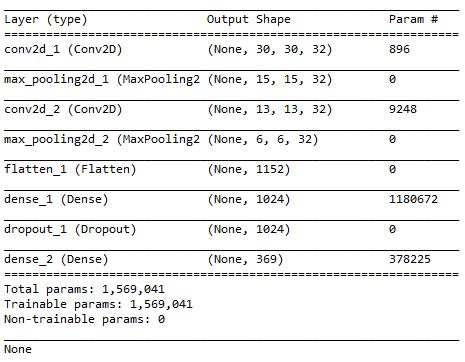
\includegraphics[width=1\textwidth]{figures/huda/chapter7/17.JPG}}
	\caption{In[10]}
	\label{c7_17}
\end{figure}
\item Jelaskan kode program pada blok \# In[11]
\par Berikut adalah kode program yang digunakan :
\lstinputlisting[firstline=89, lastline=90, caption=Kode Program 11, label={11}]{src/MathSymbols.py}
\par Dari kode listing pada kode program 11, dapat dijelaskan seperti berikut :
\begin{itemize}
\item Impor Modul Callbacks dari Librari Keras.
\item Variabel callback mendefinisikan Callback ini untuk menulis log untuk TensorBoard, yang memungkinkan Anda untuk memvisualisasikan grafik dinamis dari pelatihan dan metrik pengujian Anda, serta histogram aktivasi untuk berbagai lapisan dalam model Anda.
\end{itemize}
\par Sehingga dari kode program tersebut bila dijalankan, maka menghasilkan seperti pada gambar \ref{c7_18}.
\begin{figure}[!htbp]
	\centerline{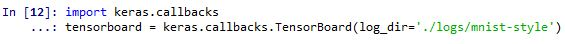
\includegraphics[width=1\textwidth]{figures/huda/chapter7/18.JPG}}
	\caption{In[11]}
	\label{c7_18}
\end{figure}
\item Jelaskan kode program pada blok \# In[12]
\par Berikut adalah kode program yang digunakan :
\lstinputlisting[firstline=93, lastline=102, caption=Kode Program 12, label={12}]{src/MathSymbols.py}
\par Dari kode listing pada kode program 12, dapat dijelaskan seperti berikut :
\begin{itemize}
\item Melakukan fit model dengan 32 ukuran subset dari sampel pelatihan Anda
\item Epoch sebanyak 10 kali
\item Vebrose=2 maksudnya menampilkan nomor dari epoch yang sedang berjalan atau yang sudah dijalankan.
\item Validasi plit sebanayk 20\% sebagai fraksi data pelatihan untuk digunakan sebagai data validasi.
\item Menggunakan TensorBoard sebagai callback untuk diterapkan selama pelatihan dan validasi.
\item Variabel score mengembalikan nilai evaluate untuk menampilkan data lost dan data accuracy dari test
\item Menampilkan data loss dengan menghitung jumlah kemunculan nol .
\item Menampilkan data accuracy dengan menghitung jumlah kemunculan 1.
\end{itemize}
\par Sehingga dari kode program tersebut bila dijalankan, maka menghasilkan seperti pada gambar \ref{c7_19}.
\begin{figure}[!htbp]
	\centerline{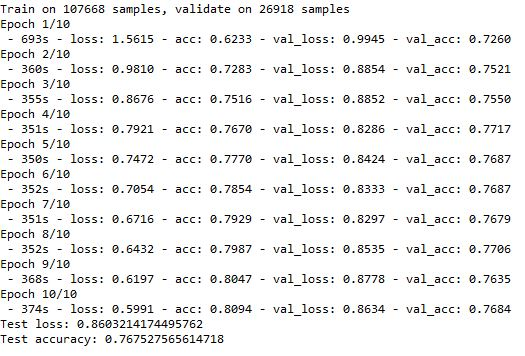
\includegraphics[width=1\textwidth]{figures/huda/chapter7/19.JPG}}
	\caption{In[12]}
	\label{c7_19}
\end{figure}
\item Jelaskan kode program pada blok \# In[13]
\par Berikut adalah kode program yang digunakan :
\lstinputlisting[firstline=106, lastline=137, caption=Kode Program 13, label={13}]{src/MathSymbols.py}
\par Dari kode listing pada kode program 13, dapat dijelaskan seperti berikut :
\begin{itemize}
\item impor modul time dari python anaconda
\item Variabel result berisikan array kosong.
\item Menggunakan convolution 2D yang dimana akan memiliki 1 atau 2 layer.
\item Mendefinisikan dense\_size dengan ukuran 128, 256, 512, 1024, 2048
\item Mendefinsikan drop\_out dengan 0, 25\%, 50\%, dan 75\%
\item Melakukan pemodelan Sequential
\item Jika ini adalah layer pertama, kita perlu memasukkan bentuk input.
\item Kalau tidak kita hanya akan menambahkan layer.
\item Kemudian, setelah menambahkan layer konvolusi, kita akan melakukan hal yang sama dengan max pooling.
\item  Lalu, kita akan meratakan atau flatten dan menambahkandense size ukuran apa pun yang berasal dari dense\_size. Dimana akan selalu menggunakan algoritma tanh
\item Jika dropout digunakan, kita akan menambahkan layer dropout. Menyebut dropout ini berarti, katakanlah 50\%, bahwa setiap kali ia memperbarui bobot setelah setiap batch, ada peluang 50\% untuk setiap bobot yang tidak akan diperbarui
\item menempatkan ini di antara dua lapisan padat untuk dihidupkan dari melindunginya dari overfitting.
\item  Lapisan terakhir akan selalu menjadi jumlah kelas karena itu harus, dan menggunakan softmax. Itu dikompilasi dengan cara yang sama.
\item Atur direktori log yang berbeda untuk TensorBoard sehingga dapat membedakan konfigurasi yang berbeda.
\item Variabel start akan memanggil modul time atau waktu
\item Melakukan fit atau compile 
\item MElakukan scoring dengan .evaluate yang akan menampilkan data loss dan accuracy dari model
\item end merupakan variabel untuk melihat waktu akhir pada saat pemodelan berhasil dilakukan.
\item Menampilkan hasil dari run skrip diatas
\end{itemize}
\par Sehingga dari kode program tersebut bila dijalankan, maka menghasilkan seperti pada gambar \ref{c7_20}.
\begin{figure}[!htbp]
	\centerline{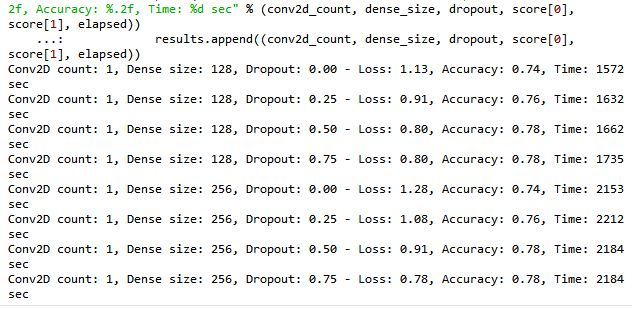
\includegraphics[width=1\textwidth]{figures/huda/chapter7/20.JPG}}
	\caption{In[13]}
	\label{c7_20}
\end{figure}
\item Jelaskan kode program pada blok \# In[14]
\par Berikut adalah kode program yang digunakan :
\lstinputlisting[firstline=141, lastline=151, caption=Kode Program 14, label={14}]{src/MathSymbols.py}
\par Dari kode listing pada kode program 14, dapat dijelaskan seperti berikut :
\begin{itemize}
\item Melakukan pemodelan Sequential
\item Untuk layer pertama, Menambahkan Convolutio 2D dengan dmensi 32, dan ukuran matriks 3x3 dengan function aktivasi yang digunakan yaitu relu dan menampilkan input\_shape
\item Dilakukan Max Pooling 2D dengan ukuran matriks 2x2
\item Untuk layer kedua, melakukan Convolusi lagi dengan kriteria yang sama tanpa menambahkan input, ini dilakukan untuk mendapatkan data yang terbaik
\item Flatten digubakan ntuk meratakan inputan
\item Menambahkan dense input sebanyak 128 neuron dengan menggunakan function aktivasi tanh.
\item Dropout sebanyak 50\% untuk menghindari overfitting
\item Menambahkan dense pada model untuk output dimana layer ini akan menjadi jumlah dari class yang ada.
\item Mengcompile model yang didefinisikan diatas
\item Menampilkan ringkasan dari pemodelan yang dilakukan
\end{itemize}
\par Sehingga dari kode program tersebut bila dijalankan, maka menghasilkan seperti pada gambar \ref{c7_21}.
\begin{figure}[!htbp]
	\centerline{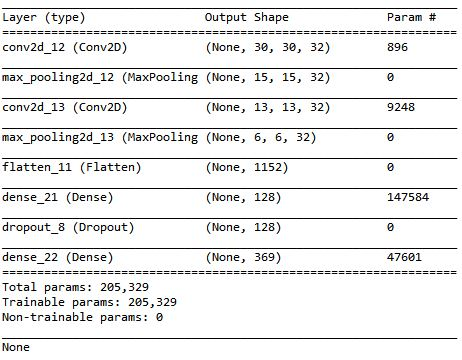
\includegraphics[width=1\textwidth]{figures/huda/chapter7/21.JPG}}
	\caption{In[14]}
	\label{c7_21}
\end{figure}
\item Jelaskan kode program pada blok \# In[15]
\par Berikut adalah kode program yang digunakan :
\lstinputlisting[firstline=153, lastline=155, caption=Kode Program 15, label={15}]{src/MathSymbols.py}
\par Dari kode listing pada kode program 15, dapat dijelaskan seperti berikut :
\begin{itemize}
\item Melakukan fit dengan join data train dan test agar dapat dilakukan pelatihan untuk jaringan pada smeua data yang dimiliki.
\end{itemize}
\par Sehingga dari kode program tersebut bila dijalankan, maka menghasilkan seperti pada gambar \ref{c7_22}.
\begin{figure}[!htbp]
	\centerline{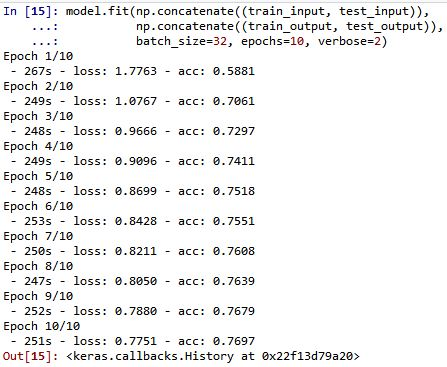
\includegraphics[width=1\textwidth]{figures/huda/chapter7/22.JPG}}
	\caption{In[15]}
	\label{c7_22}
\end{figure}
\item Jelaskan kode program pada blok \# In[16]
\par Berikut adalah kode program yang digunakan :
\lstinputlisting[firstline=158, lastline=158, caption=Kode Program 16, label={16}]{src/MathSymbols.py}
\par Dari kode listing pada kode program 16, dapat dijelaskan seperti berikut :
\begin{itemize}
\item Menyimpan atau save model yang telah di latih dengan nama mathsymbols.model 
\end{itemize}
\par Sehingga dari kode program tersebut bila dijalankan, maka menghasilkan seperti pada gambar \ref{c7_23}.
\begin{figure}[!htbp]
	\centerline{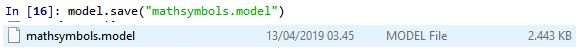
\includegraphics[width=1\textwidth]{figures/huda/chapter7/23.JPG}}
	\caption{In[16]}
	\label{c7_23}
\end{figure}
\item Jelaskan kode program pada blok \# In[17]
\par Berikut adalah kode program yang digunakan :
\lstinputlisting[firstline=161, lastline=161, caption=Kode Program 17, label={17}]{src/MathSymbols.py}
\par Dari kode listing pada kode program 17, dapat dijelaskan seperti berikut :
\begin{itemize}
\item Simpan label enkoder (untuk membalikkan one-hot encoder) dengan nama classes.npy
\end{itemize}
\par Sehingga dari kode program tersebut bila dijalankan, maka menghasilkan seperti pada gambar \ref{c7_24}.
\begin{figure}[!htbp]
	\centerline{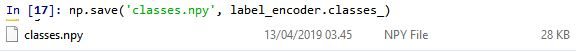
\includegraphics[width=1\textwidth]{figures/huda/chapter7/24.JPG}}
	\caption{In[17]}
	\label{c7_24}
\end{figure}
\item Jelaskan kode program pada blok \# In[18]
\par Berikut adalah kode program yang digunakan :
\lstinputlisting[firstline=167, lastline=169, caption=Kode Program 18, label={18}]{src/MathSymbols.py}
\par Dari kode listing pada kode program 18, dapat dijelaskan seperti berikut :
\begin{itemize}
\item Impor models dari librari Keras
\item Variabel model2 akan memanggil model yang telah disave tadi 
\item Menampilkan ringkasan dari hasil pemodelan
\end{itemize}
\par Sehingga dari kode program tersebut bila dijalankan, maka menghasilkan seperti pada gambar \ref{c7_25}.
\begin{figure}[!htbp]
	\centerline{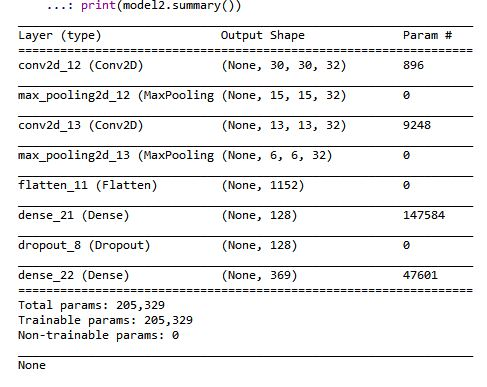
\includegraphics[width=1\textwidth]{figures/huda/chapter7/25.JPG}}
	\caption{In[18]}
	\label{c7_25}
\end{figure}
\item Jelaskan kode program pada blok \# In[19]
\par Berikut adalah kode program yang digunakan :
\lstinputlisting[firstline=172, lastline=184, caption=Kode Program 19, label={19}]{src/MathSymbols.py}
\par Dari kode listing pada kode program 19, dapat dijelaskan seperti berikut :
\begin{itemize}
\item Memanggil fungsi LabelEncoder
\item Variabel label\_encoder akan memanggil class yang disave sebelumnya.
\item Function Predict akan mengubah gambar kedalam bentuk array
\item Variabel prediction akan melakukan prediksi untuk model2 dengan reshape variabel newimg dengan bentukarray 4D.
\item Variabel inverted akan mencari nilai tertinggi output dari hasil prediksi tadi
\item Menampilkan hasil dari variabel prediction dan inverted
\end{itemize}
\par Sehingga dari kode program tersebut bila dijalankan, maka menghasilkan seperti pada gambar \ref{c7_26}.
\begin{figure}[!htbp]
	\centerline{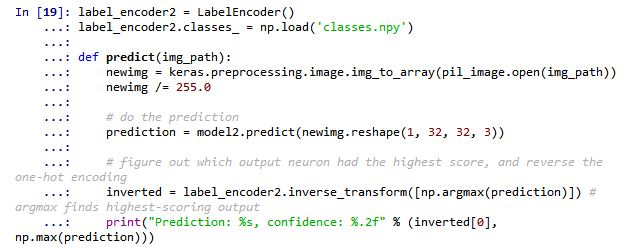
\includegraphics[width=1\textwidth]{figures/huda/chapter7/26.JPG}}
	\caption{In[19]}
	\label{c7_26}
\end{figure}
\item Jelaskan kode program pada blok \# In[20]
\par Berikut adalah kode program yang digunakan :
\lstinputlisting[firstline=187, lastline=191, caption=Kode Program 20, label={20}]{src/MathSymbols.py}
\par Dari kode listing pada kode program 20, dapat dijelaskan seperti berikut :
\begin{itemize}
\item Melakukan prediksi dari pelatihan dari gambar v2-00010.png
\item Melakukan prediksi dari pelatihan dari gambar v2-00500.png
\item Melakukan prediksi dari pelatihan dari gambar v2-00700.png
\end{itemize}
\par Sehingga dari kode program tersebut bila dijalankan, maka menghasilkan seperti pada gambar \ref{c7_27}.
\begin{figure}[!htbp]
	\centerline{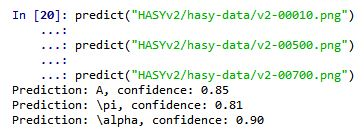
\includegraphics[width=1\textwidth]{figures/huda/chapter7/27.JPG}}
	\caption{In[20]}
	\label{c7_27}
\end{figure}
\end{enumerate}

\subsection{Penanganan Eror}
\begin{enumerate}
\item skrinsut error
\begin{figure}[!htbp]
	\centerline{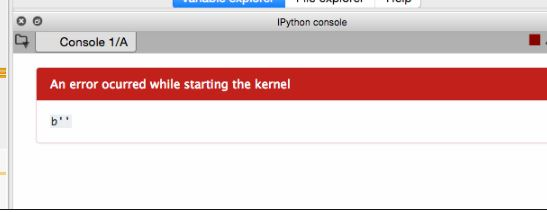
\includegraphics[width=1\textwidth]{figures/huda/chapter7/eror.JPG}}
	\caption{Eror}
	\label{c7_28}
\end{figure}
\item Tuliskan kode eror dan jenis errornya
\subitem Eror tersebut merupakan eror yang terjadi dan membuat kita tidak dapat mengakses dan menggunakan kernel atau konsol pada spyder.
\item Solusi pemecahan masalah error tersebut
\begin{itemize}
\item Tutup spyder yang sedang dijalankan
\item Kemudian buka kembali spyder
\item maka eror pada kernel tersebut akan hilang dan kembali stabil agar bisa mengakses konsol tersebut.
\end{itemize}
\end{enumerate}